\subsection*{Eigenvalue Problems}

If \iMbox{A} is \underline{diagonalizable} then \underline{eigen-decomposition} is \iMbox{A = X \Lambda X^{-1}}

\begin{itemize}

      \item
            \textbf{Dominant} \iMbox{\lambda_{1};\mathbf{x}_{1}} are such that
            \iMbox{\lvert \lambda_{1} \rvert} is \underline{strictly largest} for which
            \iMbox{A\mathbf{x} = \lambda \mathbf{x}}
            \tcbbreak
      \item
            \textbf{Rayleigh quotient} for \underline{Hermitian} \iMbox{A = A ^{\dagger}} is
            \iMbox{ R_A(\mathbf{x}) = \frac{\mathbf{x}^{\dagger}A\mathbf{x}}{\mathbf{x}^{\dagger}\mathbf{x}}}

            \begin{itemize}

                  \item
                        \underline{Eigenvectors} are \underline{stationary points} of \iMbox{ R_{A}}
                  \item
                        \iMbox{ R_{A}(\mathbf{x})} is \underline{closest} to being \underline{like eigenvalue}
                        of \iMbox{\mathbf{x}}, i.e. \iMbox{ R_{A}(\mathbf{x})=\underset{\alpha}{\operatorname{argmin}}\|A \mathbf{x}-\alpha \mathbf{x}\|_2}
                  \item
                        \iMbox{ R_{A}(\mathbf{x}) - R_{A}(\nu) = O(\lVert \mathbf{x} - \nu \rVert^{2})}
                        as \iMbox{\mathbf{x} \to \nu} where \iMbox{\nu} is \underline{eigenvector}
            \end{itemize}
\end{itemize}

\hSep % ---

\textbf{Power iteration}: define sequence
\iMbox{ \mathbf{b}^{(k+1)}=\frac{A \mathbf{b}^{(k)}}{\left\|A \mathbf{b}^{(k)}\right\|}}
with \underline{initial} \iMbox{\mathbf{b}^{(0)}} s.t. \iMbox{\lVert \mathbf{b}^{(0)} \rVert = 1}
\begin{itemize}
      \item
            Assume \textbf{dominant} \iMbox{\lambda_{1};\mathbf{x}_{1}} exist
            for \iMbox{A}, and that
            \iMbox{ \mathrm{proj}_{\mathbf{x}_{1}}\left(\mathbf{b}^{(0)} \right) \neq \mathbf{0}}
      \item
            Under above assumptions,
            \iMbox{ \mu_{k} = R_A\left(\mathbf{b}^{(k)} \right) = \frac{{\mathbf{b}^{(k)}}^{\dagger}A\mathbf{b}^{(k)}}{{\mathbf{b}^{(k)}}^{\dagger}\mathbf{b}^{(k)}}}
            converges to \textbf{dominant \iMbox{\lambda_{1}}}
      \item
            \iMbox{\langle\mathbf{b}_{k}\rangle} converges to some
            \textbf{dominant} \iMbox{\mathbf{x}_{1}} associated with
            \iMbox{\lambda_{1}} =>
            \iMbox{ \left\|A \mathbf{b}^{(k)}\right\|} converges to
            \iMbox{|\lambda_{1}|}
      \item
            If \iMbox{ \mathrm{proj}_{\mathbf{x}_{1}}\left(\mathbf{b}^{(0)} \right) =\mathbf{0}}
            then \iMbox{\langle\mathbf{b}_{k}\rangle;\langle \mu_{k}\rangle}
            converge to \underline{second} \textbf{dominant} \iMbox{\lambda_{2};\mathbf{x}_{2}} instead
      \item
            If \textbf{no dominant \iMbox{\lambda}} \emph{(i.e. multiple
                  eigenvalues of maximum \iMbox{|\lambda|})} then
            \iMbox{\langle\mathbf{b}_{k}\rangle} will converge to \underline{linear combination}
            of their corresponding \underline{eigenvectors}
      \item
            Slow convergence if \textbf{dominant \iMbox{\lambda_{1}}} not \underline{``very dominant''}
      \item
            \iMbox{ \lVert \mathbf{b}^{(k)} - \alpha_{k}\mathbf{x}_{1} \rVert = O\left( \left\lvert  \frac{\lambda_{2}}{\lambda_{1}}  \right\rvert^k \right)}
            for \textbf{phase factor} \iMbox{\alpha_{k} \in \{ -1,1 \}} it may \underline{alternate} if \iMbox{\lambda_{1}<0}
            \begin{itemize}

                  \item
                        \iMbox{ \alpha_{k} = \frac{(\lambda_{1})^k c_{1}}{|\lambda_{1}|^k |c_{1}|}}
                        where \iMbox{ c_{1} = \mathbf{x}_{1}^{\dagger}\mathbf{b}^{(0)}} and assuming
                        \iMbox{\mathbf{b}^{(k)};\mathbf{x}_{1}} are \underline{normalized}
            \end{itemize}
      \item
            \iMbox{(A - \sigma I)} has \textbf{eigenvalues} \iMbox{\lambda-\sigma}

            => \underline{power-iteration} on \iMbox{(A - \sigma I)} has \iMbox{\frac{\lambda_{2}-\sigma}{\lambda_{1}-\sigma}}
      \item
            Eigenvector guess => estimated eigenvalue
\end{itemize}

\hSep % ----

\textbf{Inverse (power-)iteration}: perform \underline{power iteration} on
\iMbox{ (A - \sigma I)^{-1}} to get \iMbox{\lambda_{1,\sigma}} \textbf{closest} to \iMbox{\sigma}
\begin{itemize}

      \item
            \iMbox{(A - \sigma I)^{-1}} has \underline{eigenvalues}
            \iMbox{(\lambda- \sigma)^{-1}} so \underline{power iteration} will yield
            \textbf{largest \iMbox{(\lambda_{1,\sigma}- \sigma)^{-1}}}
      \item
            i.e. will yield \textbf{smallest
                  \iMbox{\lambda_{1,\sigma}- \sigma}}, i.e. will yield
            \iMbox{\lambda_{1,\sigma}} \textbf{closest} to \iMbox{\sigma}
      \item
            \iMbox{ \lVert \mathbf{b}^{(k)} - \alpha_{k}\mathbf{x}_{1,\sigma} \rVert = O\left( \left\lvert  \frac{\lambda_{1,\sigma} - \sigma}{\lambda_{2,\sigma} - \sigma}  \right\rvert^k \right)}
            where \iMbox{\mathbf{x}_{1,\sigma}} corresponds to
            \iMbox{\lambda_{1,\sigma}} and \iMbox{ \lambda_{2,\sigma}} is \underline{2nd-closest} to \iMbox{\sigma}
      \item
            Efficiently compute \underline{eigenvectors} for \textbf{known eigenvalues}
            \iMbox{\sigma}
      \item
            Eigenvalue guess => estimated eigenvector

            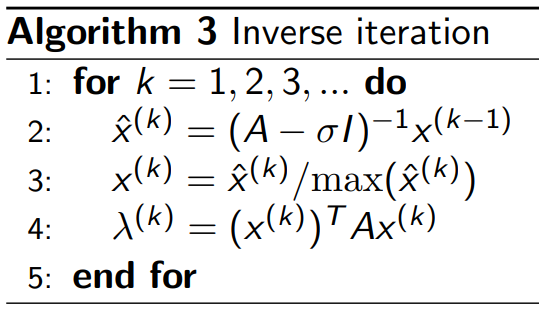
\includegraphics[width=60pt]{inviter}
      \item
            Can reduce matrix inversion \iMbox{O(m^3)} to \iMbox{O(m^2)} by
            pre-factorization
\end{itemize}


\subsection*{Nonlinear Systems of Equations}

\underline{Recall} that \iMbox{ \nabla f(\mathbf{x})} is direction of \textbf{max.}
rate-of-change \iMbox{ \lvert \nabla f(\mathbf{x}) \rvert}

\underline{Idea:} Search for \underline{stationary point} by \textbf{gradient descent}:
\iMbox{ \mathbf{x}^{(k+1)} = \mathbf{x}^{(k)} - \alpha \nabla f(\mathbf{x}^{(k)})}
for \underline{step length} \iMbox{\alpha}

\hSep % ---

If \iMbox{A} is \underline{positive-definite}, solving \iMbox{A\mathbf{x} = \mathbf{b}} and
\iMbox{ \min_{\mathbf{x}} f(\mathbf{x}) = \frac{1}{2} \mathbf{x}^T A \mathbf{x} - \mathbf{x}^T \mathbf{b}}
are equivalent


Get \underline{iterative methods}
\iMbox{ \mathbf{x}^{(k+1)} = \mathbf{x}^{(k)} - \alpha^{(k)} \mathbf{p}^{(k)}}
for \underline{step length} \iMbox{\alpha^{(k)}} and \underline{directions} \iMbox{\mathbf{p}^{(k)}}

\hSep % ---

\textbf{Conjugate gradient (CG) method}: if \iMbox{A \in \mathbb{R}^{n \times n}} \underline{symmetric} then
\iMbox{ \langle \mathbf{u},\mathbf{v} \rangle_{A} = \mathbf{u}^T A\mathbf{v}}
is an \underline{inner-product}
\begin{itemize}

      \item
            \textbf{GC} chooses \iMbox{ \mathbf{p}^{(k)}} that are \underline{conjugate}
            w.r.t. \iMbox{A},
            i.e. \iMbox{ \langle \mathbf{p}^{(i)},\mathbf{p}^{(j)} \rangle_{A} = 0}
            for \iMbox{i\neq j}
      \item
            And chooses \iMbox{\alpha^{(k)}} s.t. \textbf{residuals}
            \iMbox{ \mathbf{r}^{(k)} = - {\nabla f}(\mathbf{x}^{(k)}) = \mathbf{b} - A\mathbf{x}^{(k)}}
            are \underline{orthogonal}

            \begin{itemize}

                  \item
                        \iMbox{k=0} =>
                        \iMbox{ \mathbf{p}^{(0)} = - {\nabla f}(\mathbf{x}^{(0)}) = \mathbf{r}^{(0)}}
                  \item
                        \iMbox{k\geq 1} =>
                        \iMbox{ \mathbf{p}^{(k)} = \mathbf{r}^{(k)} - \sum_{i<k} {\frac{\langle \mathbf{p}^{(i)},\mathbf{r}^{(k)} \rangle_{A}}{\langle \mathbf{p}^{(i)},\mathbf{p}^{(i)} \rangle_{A}}\mathbf{p}^{(i)}}}
                  \item
                        \iMbox{ \alpha^{(k)} = \mathrm{argmin}_{\alpha} {f(\mathbf{x}^{(k)} + \alpha^{(k)} \mathbf{p}^{(k)})} = \frac{\mathbf{p}^{(k)} \cdot \mathbf{r}^{(k)}}{\langle \mathbf{p}^{(k)},\mathbf{p}^{(k)} \rangle_{A}}}
            \end{itemize}
      \item
            \underline{Without rounding errors}, \textbf{CG} converges in \iMbox{\leq n} iterations
            \tcbbreak

            \begin{itemize}

                  \item
                        Similar to to \underline{Gram-Schmidt} \emph{(but different inner-product)}
                  \item
                        \iMbox{\langle \mathbf{p}^{(0)},\dots,\mathbf{p}^{(n-1)} \rangle} and
                        \iMbox{\langle \mathbf{r}^{(0)},\dots,\mathbf{r}^{(n-1)} \rangle}
                        are \underline{bases} for \iMbox{\mathbb{R}^{n}}
            \end{itemize}
\end{itemize}


\subsection*{\texorpdfstring{QR Algorithm to find Schur decomposition
            \iMbox{A = QUQ^{\dagger}}}{QR Algorithm to find Schur decomposition }}


Any \iMbox{A \in \mathbb{C}^{m \times m}} has 
\textbf{Schur decomposition} \iMbox{A = QUQ^{\dagger}}
\begin{itemize}

      \item
            \iMbox{Q} is unitary, i.e.~\iMbox{Q^{\dagger} = Q^{-1}} and
            upper-triangular \iMbox{U}
      \item
            Diagonal of \iMbox{U} contains \textbf{eigenvalues} of \iMbox{A}
\end{itemize}

\hSep % ---

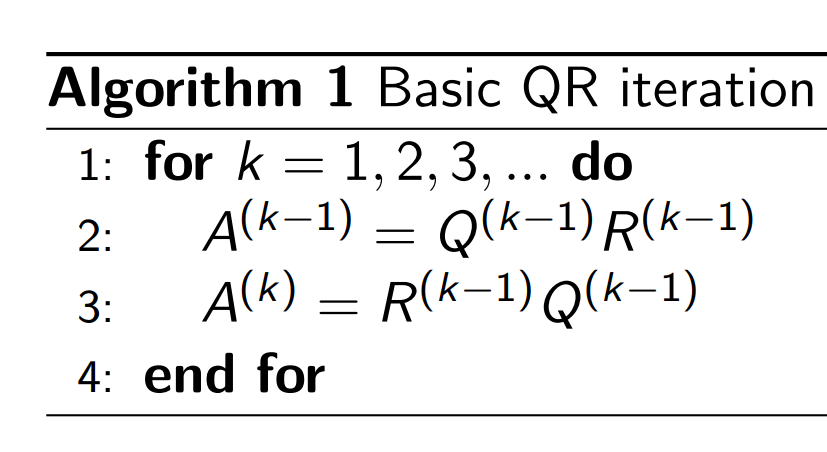
\includegraphics[width=75pt]{qralg}

\begin{itemize}

      \item For \iMbox{A \in \mathbb{R}^{m \times m}} each iteration
            \iMbox{ A^{(k)} = Q^{(k)}R^{(k)}} produces orthogonal
            \iMbox{{Q^{(k)}}^{T} = {Q^{(k)}}^{-1}}

      \item So \iMbox{ 
            \begin{aligned}
                  A^{(k+1)}=R^{(k)} Q^{(k)}
                  &= ({Q^{(k)}}^{T} Q^{(k)}) R^{(k)} Q^{(k)}
                  \\ &={Q^{(k)}}^{T} A^{(k)} Q^{(k)}
            \end{aligned}
      }
            means \iMbox{A^{(k+1)}} is \textbf{similar} to \iMbox{A^{(k)}}

      \item Setting \iMbox{ A^{(0)} = A} we get
            \iMbox{A^{(k)} = (\tilde{Q}^{(k)})^{T} A \tilde{Q}^{(k)}} where
            \iMbox{\tilde{Q}^{(k)} = Q^{(0)}\cdots Q^{(k-1)}}
      
      \item Under \underline{certain conditions} \textbf{QR algorithm} converges to
            \textbf{Schur decomposition}
\end{itemize}

\hSep % ---

We can \textbf{apply shift} \iMbox{\mu^{(k)}} at \underline{iteration} \iMbox{k}

=> \iMbox{ A^{(k)} - \mu^{(k)}I = Q^{(k)}R^{(k)}; \ A^{(k+1)} = R^{(k)}Q^{(k)} + \mu^{(k)}I}
\begin{itemize}

      \item
            If \textbf{shifts} are \underline{good eigenvalue estimates} then \underline{last column} of
            \iMbox{\tilde{Q}^{(k)}} converges \underline{quickly} to an \textbf{eigenvector}
      \item
            Estimate \iMbox{\mu^{(k)}} with \underline{Rayleigh quotient} =>
            \iMbox{ \mu^{(k)} = (A_{k})_{mm} = (\tilde{\mathbf{q}}^{(k)}_{m})^{T} A \tilde{\mathbf{q}}^{(k)}_{m}}
            where \iMbox{\tilde{\mathbf{q}}^{(k)}_{m}} is \iMbox{m}-th column of
            \iMbox{\tilde{Q}^{(k)}}

\end{itemize}